\documentclass[11pt,twocolumn]{article}
\usepackage[margin=0.85in]{geometry}
\usepackage{amsmath,amssymb}
\usepackage{booktabs}
\usepackage{graphicx}
\usepackage[hidelinks]{hyperref}
\usepackage{stix}

\newcommand{\gw}{\textsc{gradwave}}
\newcommand{\qe}{\textsc{Quantum ESPRESSO}}

\title{\gw: differentiable plane-wave density functional theory in PyTorch}
\author{Will Laderer}
\date{July 2026}

\begin{document}
\maketitle

\begin{abstract}
We present \gw, a plane-wave pseudopotential density functional theory code
in which every energy term is a differentiable PyTorch function of its
inputs. The code reproduces \qe{} 7.5 at the precision established for
mature plane-wave codes. Equation-of-state comparisons over six solids give
$\Delta \leq 0.17$ meV/atom, lattice constants agree to $4\times10^{-4}$
\AA{}, and a 0.5 ps microcanonical trajectory driven by autograd forces
conserves total energy to a secular drift near 1 $\mu$eV/atom. On matched
small cells the code runs within a factor of three of \qe{} on a consumer
GPU. The differentiable formulation then supplies derivatives that
conventional codes obtain only from hand-derived, functional-specific
implementations. Gradients of the total energy with respect to
exchange-correlation parameters match self-consistent finite differences to
$3\times10^{-10}$ and support direct fitting of functional parameters. The
Hubbard $U$ becomes both a differentiable parameter, through an exact
$dE/dU$, and a self-determined one, through a linear-response implementation
whose interacting susceptibility is screened by an exchange-correlation
kernel evaluated as an automatic second derivative. The same kernel drives
electric-field response, and the resulting dielectric constants and Born
charges agree with \texttt{ph.x} to 0.002\% for Si and to 0.3\% or better
for MgO. Phonon frequencies from displaced autograd forces agree with
density functional perturbation theory to 0.15\%. Noncollinear magnetism
uses an exchange field generated by the same automatic differentiation, and
spin-orbit benchmarks reproduce the GaAs split-off gap to 0.03 meV.
\end{abstract}

\section{Introduction}

Plane-wave density functional theory (DFT) rests on a small number of
derivative relationships. Forces are derivatives of the total energy with
respect to atomic positions, the exchange-correlation (XC) potential is a
functional derivative of the XC energy, phonons and dielectric constants are
second derivatives, and the Hubbard $U$ of DFT+$U$ is itself defined through
a derivative of occupations with respect to a probe potential
\cite{baroni2001,cococcioni2005}. Production codes implement each of these
by hand. Every new functional requires a new $v_{\rm xc}$ and a new
$f_{\rm xc}$, every new perturbation requires new matrix elements, and the
implementations are validated against one another rather than against the
energy expression they differentiate.

Automatic differentiation removes this duplication. If the total energy is
a differentiable program, then its gradients with respect to any input,
namely positions, XC parameters, occupation-matrix probes, or external
fields, are exact by construction and are produced by the same code path
that evaluates the energy. Prior work has demonstrated this principle for
Hartree-Fock and for basis-set and orbital-free DFT
\cite{tamayo2018,kasim2021}. The question we address is whether a
differentiable formulation can meet the precision and performance standards
of established plane-wave codes on periodic solids, including metals,
magnetism, spin-orbit coupling, and DFT+$U$, and what the derivative capabilities provide once it does.

\gw{} answers the first part by direct comparison against \qe{} 7.5
\cite{giannozzi2020} at identical pseudopotentials, cutoffs, $k$-meshes, and
fast Fourier transform (FFT) grids. Section~\ref{sec:validation} reports
equation-of-state, molecular-dynamics, and response-function benchmarks, and
Sec.~\ref{sec:speed} reports wall-clock comparisons. The second part is
addressed in Sec.~\ref{sec:derivs}, which collects four capabilities that
follow from the computation graph. These are exact gradients with respect
to XC parameters, a differentiable and self-determined Hubbard $U$, phonons
from autograd forces, and noncollinear magnetism with an automatically
generated exchange field.

\section{Implementation}
\label{sec:impl}

\gw{} implements norm-conserving pseudopotential DFT in the
Kleinman-Bylander form with UPF~v2 inputs (ONCV and PseudoDojo sets
\cite{hamann2013,schlipf2015,vansetten2018}), LDA and PBE functionals
\cite{pbe1996}, Monkhorst-Pack sampling with space-group reduction,
Gaussian, Marzari-Vanderbilt, and Methfessel-Paxton smearing, collinear
spin, and noncollinear spinors with spin-orbit coupling from fully
relativistic $j$-resolved projectors. All arithmetic is float64 or
complex128, on CPU or a single GPU. All results below were obtained on a
laptop with 22 hardware threads and an NVIDIA RTX 3050 with 6 GB of memory.

The code is organized so that automatic differentiation never traces the
self-consistent field (SCF) loop. A pure tensor layer expresses every
energy term and the Hamiltonian apply as differentiable functions. A solver
layer runs Davidson diagonalization and Pulay mixing under
\texttt{torch.no\_grad()}. Derivatives are then taken at the converged
fixed point in one of three ways. Quantities protected by stationarity,
such as forces and $dE/d\theta$ for any energy parameter $\theta$, are
partial derivatives at fixed density and orbitals and cost one backward
pass. Quantities that require the density response are computed from
conduction-projected Sternheimer equations, in which the Hartree-XC kernel
$f_{\rm Hxc}$ is applied as a Hessian-vector product of the XC energy by
double backpropagation, so no kernel is ever derived by hand. Mixed second
derivatives combine the two, with one response solve and one backward pass.

The XC functional is a \texttt{torch.nn.Module}. Its potential, its kernel,
and its parameter gradients all come from the same energy expression, so a
functional with trainable parameters participates in every capability of
the code, including the response solvers, without additional
implementation.

\section{Agreement with Quantum ESPRESSO}
\label{sec:validation}

\begin{figure*}[t]
\centering
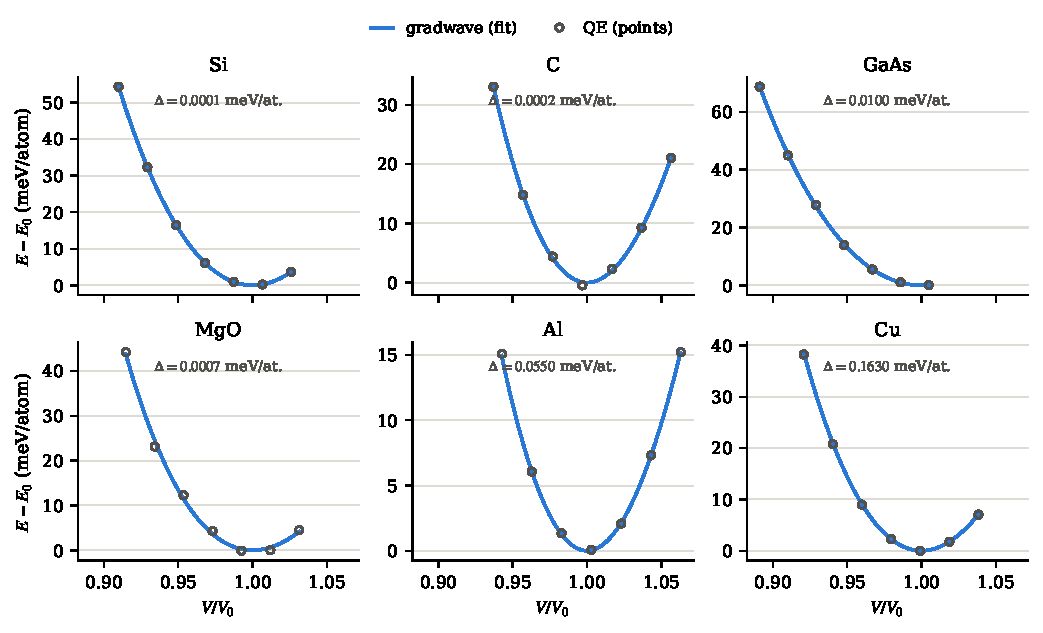
\includegraphics[width=\textwidth]{figs/fig_eos.pdf}
\caption{Equations of state for six solids at seven volumes spanning
$\pm 6\%$, computed with PBE and ONCV pseudopotentials at identical
cutoffs, $k$-meshes, and FFT grids in both codes. Solid lines show
Birch-Murnaghan fits to the \gw{} energies and open circles show the \qe{}
energies. The $\Delta$ value in each panel is the root-mean-square
difference between the two fitted curves over the volume window
\cite{lejaeghere2016}.}
\label{fig:eos}
\end{figure*}

The primary validation target is the equation-of-state comparison of
Lejaeghere \textit{et al.} \cite{lejaeghere2016}, in which two codes are
compared through the root-mean-square difference $\Delta$ of their fitted
energy-volume curves. Total energies were computed at seven volumes
spanning $\pm 6\%$ for Si, C, GaAs, MgO, Al, and Cu with PBE, ONCV
pseudopotentials, and converged cutoffs of 50 to 90 Ry, and Birch-Murnaghan
forms were fitted to both data sets. Figure~\ref{fig:eos} shows the result.
$\Delta$ is at or below 0.17 meV/atom for all six solids and at or below
0.01 meV/atom for the four insulators, against a range of 0.3 to 1 meV/atom
reported among mature plane-wave codes \cite{lejaeghere2016}. Fitted
lattice constants agree to $4\times10^{-4}$ \AA{} and bulk moduli to 0.6
GPa. Two numerical conditions were required for smooth curves and are
recorded with the benchmark scripts. The FFT grid must be held fixed
across volumes, and the cutoff must be converged, since plane-wave shells
crossing the cutoff as the cell scales otherwise produce energy jumps that
appear identically in both codes.

\begin{figure}[t]
\centering
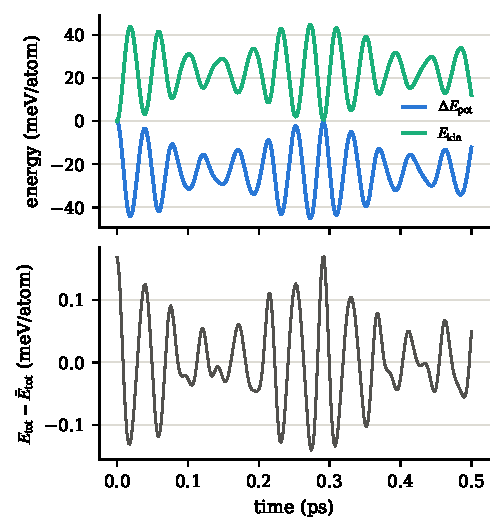
\includegraphics[width=\columnwidth]{figs/fig_nve.pdf}
\caption{Microcanonical molecular dynamics of a rattled Si$_8$ cell with a
2 fs time step, driven by autograd Hellmann-Feynman forces through the ASE
calculator on the GPU. The upper panel shows the exchange between potential
and kinetic energy. The lower panel shows the deviation of the total energy
from its mean, with a root-mean-square fluctuation of 0.067 meV/atom and a
secular drift near 1 $\mu$eV/atom over the half picosecond.}
\label{fig:nve}
\end{figure}

Energy conservation in molecular dynamics is a stricter test of
force-energy consistency than any single-point force comparison, because
the trajectory integrates every systematic error. Figure~\ref{fig:nve}
shows 0.5 ps of velocity-Verlet dynamics for a rattled Si$_8$ cell at an
average temperature of 180 K. Potential and kinetic energy exchange
roughly 45 meV/atom while the total energy fluctuates with a
root-mean-square amplitude of 0.067 meV/atom, the bounded oscillation
expected of the integrator at this time step. The secular drift, measured
as the difference between the first-half and second-half means, is 0.9
$\mu$eV/atom. The autograd force is the exact gradient of the SCF energy
surface, and the drift is at the SCF tolerance floor.

Table~\ref{tab:summary} collects the remaining benchmark
comparisons. All
were run at identical numerical settings in both codes, and the full
comparison suite of 46 integration tests passes unchanged on CPU and GPU.

\begin{table}[t]\centering
\caption{Agreement with \qe{} 7.5 at identical pseudopotentials, cutoffs,
$k$-meshes, and FFT grids.}
\label{tab:summary}
\small
\begin{tabular}{ll}
\toprule
quantity & agreement \\
\midrule
SCF energies (Si, Al, Cu, Fe, GaAs) & $\leq 2$ meV/atom \\
forces, displaced Si and Al & $\leq 5$ meV/\AA \\
Si band energies & $\leq 10$ meV \\
GaAs spin-orbit gap $\Delta_0$ & 0.3360 vs 0.3360 eV \\
NiO DFT+$U$ energy $E_U$ & 2.9956 vs 2.9942 eV \\
$\varepsilon_\infty$, Si & 23.8900 vs 23.8904 \\
Born charges, MgO & 0.07 to 0.10\% \\
Si $\Gamma$ optical phonon & 522.6 vs 523.3 cm$^{-1}$ \\
\bottomrule
\end{tabular}
\end{table}

\section{Performance}
\label{sec:speed}

\begin{figure}[t]
\centering
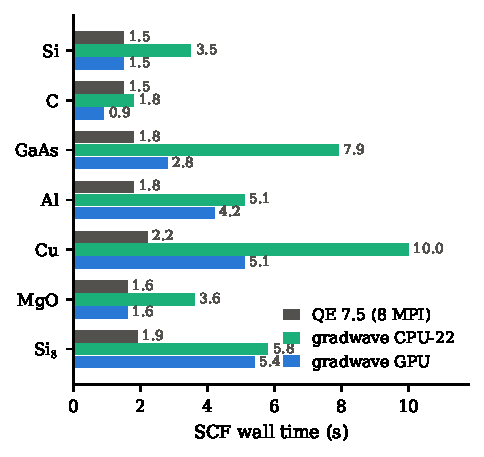
\includegraphics[width=\columnwidth]{figs/fig_speed.pdf}
\caption{SCF wall time for seven matched systems. \qe{} ran with eight MPI
ranks, and \gw{} ran on 22 CPU threads or on the RTX 3050. Cutoffs,
$k$-meshes, FFT grids, band counts, and functionals are identical, and the
converged energies agree to 1 meV/atom or better.}
\label{fig:speed}
\end{figure}

Figure~\ref{fig:speed} compares SCF wall times on seven systems with 1 to 8
atoms, with all numerical settings matched between the codes.
\qe{} completes these cells in 1.5 to 2.2 s and is faster than the \gw{}
GPU path on the metals and Si$_8$, comparable on the insulators, and 2 to
5$\times$ faster than the 22-thread CPU path. Two factors account for most
of the difference. \qe{} converges in 6 to 9 SCF iterations against 10 to
14 for \gw, which reflects mixer maturity rather than tensor throughput,
and at these sizes, below 3000 plane waves, framework overhead per
iteration is proportionally largest. The GPU advantage grows with system
size. A 78-electron Bi$_2$Se$_3$ spin-orbit calculation on an $80^3$ grid
completes its SCF in under ten minutes on the same 6 GB card. The differentiable formulation therefore remains usable for routine
ground-state work.

\section{Derivatives from the computation graph}
\label{sec:derivs}

\subsection{Exchange-correlation parameters}
\label{sec:xc}

\begin{figure*}[t]
\centering
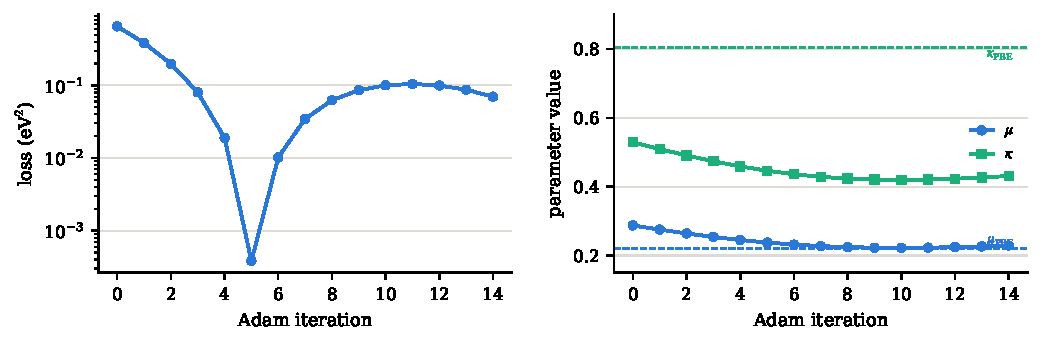
\includegraphics[width=\textwidth]{figs/fig_xc.pdf}
\caption{Fit of the learnable exchange parameters $(\kappa, \mu)$ to PBE
total energies at two silicon volumes, starting from $(0.55, 0.30)$. The
left panel shows the loss and the right panel shows the parameter
trajectories, with PBE values as dashed lines. $\mu$ converges to 0.222
against the PBE value 0.2195, while $\kappa$ drifts along a flat direction
because silicon's reduced-gradient range constrains only the $s^2$
expansion of the enhancement factor.}
\label{fig:xc}
\end{figure*}

At self-consistency the total energy is variational in the density, so the
gradient with respect to any XC parameter reduces to a partial derivative
at fixed density,
\begin{equation}
\frac{dE}{d\theta} =
\left.\frac{\partial E_{\rm xc}[\rho;\theta]}{\partial\theta}
\right|_{\rho^\star},
\end{equation}
which is one backward pass with no response solve. We verified this for a
PBE-form exchange functional with learnable $(\kappa, \mu)$, evaluated at
an off-PBE point. The autograd gradients agree with central finite
differences of full SCF re-runs to $3\times10^{-10}$ for
$\theta_\kappa$ and $7\times10^{-10}$ for $\theta_\mu$.

Figure~\ref{fig:xc} shows the gradients in use. Starting from
$(\kappa,\mu) = (0.55, 0.30)$, Adam fits the two parameters to PBE total
energies at two silicon volumes. The loss falls three orders of magnitude
in five steps, and $\mu$ converges to 0.222 against the PBE value 0.2195.
$\kappa$ does not converge, and this failure is informative. In silicon's
reduced-gradient range the enhancement factor is $F \approx 1 + \mu s^2$ to
leading order, so energy data constrain $\mu$ while $\kappa$, an $s^4$
effect, is left nearly free. The optimization performs an identifiability
analysis of the functional form on the given data. Losses that depend on
the density rather than the energy require the response of the density to
the parameters, and this path is implemented as a self-consistent adjoint
solve, validated to $2\times10^{-4}$ against finite differences.

\subsection{The Hubbard $U$}
\label{sec:u}

\gw{} implements rotationally invariant DFT+$U$ \cite{dudarev1998} with the
atomic-orbital projectors of \qe{}, validated on antiferromagnetic NiO.
The Hubbard energy agrees with \qe{} to 1.6 meV and the Ni $3d$ occupations
to $10^{-3}$. Three derivative capabilities follow.

The parameter derivative is exact and costs one backward pass. At the converged point,
\begin{equation}
\frac{dE}{dU} = \sum_{I\sigma} \tfrac12\,
{\rm Tr}\!\left[n^{I\sigma}\!\left(1 - n^{I\sigma}\right)\right],
\end{equation}
by the same stationarity argument as above. For NiO at $U = 5$ eV this
gives 0.616154 against 0.616153 from finite differences of SCF re-runs.
The force contribution of the Hubbard term follows from backpropagation
through the projector phases
$e^{-i(\mathbf{k}+\mathbf{G})\cdot\boldsymbol{\tau}}$ and matches
frozen-orbital finite differences to $5\times10^{-8}$ eV/\AA.

\begin{figure}[t]
\centering
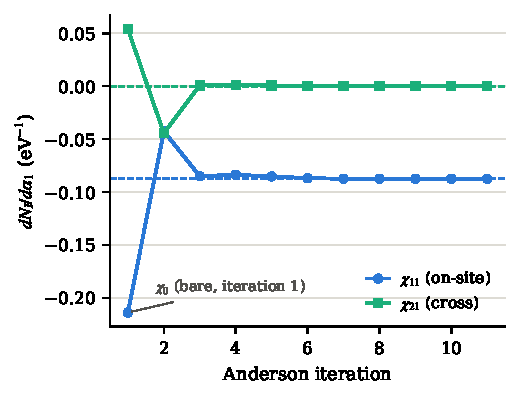
\includegraphics[width=\columnwidth]{figs/fig_uresp.pdf}
\caption{Convergence of the interacting response column
$dN_I/d\alpha_1$ for NiO under Anderson mixing. The first iteration is the
bare response $\chi_0$, computed at frozen effective potential. Dashed
lines mark the finite-difference reference values obtained from probe SCF
re-runs. Plain damped iteration diverges for this system, because the
antisymmetric magnetization mode across the two Ni sites carries a
$K\chi_0$ eigenvalue near $-6$.}
\label{fig:uresp}
\end{figure}

The linear-response $U$ of Cococcioni and de Gironcoli
\cite{cococcioni2005} is defined through occupation susceptibilities,
$U = (\chi_0^{-1} - \chi^{-1})_{II}$, conventionally evaluated by finite
differences of probe SCF calculations. \gw{} computes both
susceptibilities analytically from a single ground state. The bare
$\chi_0$ is one batched conduction-projected Sternheimer solve with the
projector probe on the right-hand side. The interacting $\chi$ screens the
probe self-consistently through the spin-resolved Hartree-XC kernel, which
is evaluated as a Hessian-vector product of $E_{\rm Hxc}$ by double
backpropagation. No $f_{\rm xc}^{\sigma\sigma'}$ was derived or coded, so
the same solver applies unchanged to any twice-differentiable spin
functional, including learnable ones. Figure~\ref{fig:uresp} shows the
convergence of the response columns. Anderson mixing \cite{anderson1965}
is required rather than optional here. PBE NiO lies near a spin instability, the antisymmetric magnetization mode across the two Ni sites
gives the iteration matrix an eigenvalue near $-6$, and plain damped
iteration diverges at any practical damping. Anderson mixing converges the
same fixed point in 11 iterations.

Table~\ref{tab:u} compares the resulting $U$ against the finite-difference
route and against the independent density functional perturbation theory
implementation in \texttt{hp.x} \cite{timrov2018}. The two \gw{} routes
agree to 0.3 meV, and both agree with \texttt{hp.x} to 0.3\%.

\begin{table}[t]\centering
\caption{Linear-response Hubbard $U$ for the Ni $3d$ manifold of NiO
(PBE, PseudoDojo, 40 Ry, $2^3$ $k$-mesh).}
\label{tab:u}
\begin{tabular}{lr}
\toprule
method & $U$ (eV) \\
\midrule
finite-difference response & 6.4493 \\
Sternheimer with autograd kernel & 6.4496 \\
\qe{} \texttt{hp.x} & 6.4308 \\
\bottomrule
\end{tabular}
\end{table}

\subsection{Phonons and electric-field response}
\label{sec:phonons}

Phonons were computed by finite displacements of $5\times10^{-3}$ \AA{}
with autograd forces, at settings matched to a \texttt{ph.x} calculation
(PBE, 40 Ry, $4^3$ mesh, $32^3$ grid). The silicon $\Gamma$ optical triplet is 522.6 cm$^{-1}$ against 523.3 cm$^{-1}$ from
perturbation theory, a 0.15\% difference, with the triplet degenerate to
the reported precision and the acoustic modes at zero under the sum rule.
Because the forces are exact gradients, the force-constant matrix is
consistent with the energy surface by construction, and the corresponding
diagonal Hessian element agrees with an energy second difference to
0.5\%.

The electric-field response uses the same Sternheimer and autograd-kernel
machinery as the Hubbard $U$. The position operator acting on Bloch
states is obtained from a solve with $\partial H/\partial k$ on the
right-hand side, where the kinetic contribution is analytic and the
nonlocal contribution is a central difference in $k$ of the projector
tables. The result is insensitive to the step over a factor-of-four range
at the sixth decimal. The dielectric constant of silicon agrees with
\texttt{ph.x} to 0.002\%. Born effective charges follow as mixed
derivatives $\partial^2 E/\partial \mathcal{E}\,\partial\tau$, in which one
backward pass through the position-differentiable pseudopotential yields
all atoms and directions per field direction. For MgO the charges agree
with \texttt{ph.x} to 0.07\% for Mg and 0.10\% for O, and the raw acoustic
sum rule violation, a $k$-mesh artifact that both codes must reproduce
before enforcement, matches as well.

\subsection{Noncollinear magnetism}
\label{sec:ncl}

The noncollinear SCF treats the exchange field the same way the collinear
code treats the potential. For a locally collinear functional the energy
depends on $(\rho, |\mathbf{m}|)$, and a single backward pass yields both
$v_{\rm xc}$ and $\mathbf{B}_{\rm xc} \parallel \mathbf{m}$, so no
functional derivative of the spin rotation was implemented. The
consequences are testable symmetries rather than fitted numbers. Spinor
iron with $\mathbf{m} \parallel \hat z$ reproduces the two-channel
collinear energy exactly at the reported precision, and rotating the
moment to $\hat x$ or to $45^\circ$ changes the total energy by 0.19
$\mu$eV in the absence of spin-orbit coupling, so the rotational
invariance of the functional emerges numerically from the automatic
field.

With fully relativistic $j$-resolved projectors the code reproduces
standard spin-orbit benchmarks. The GaAs split-off gap matches \qe{} to
0.03 meV and the free energy to 0.0007 meV/atom. For Bi$_2$Se$_3$ the
$\Gamma$-point parities of the gap-edge states swap between the
scalar-relativistic and spin-orbit calculations, with parity eigenvalues
of $\pm 1.000$ and exact Kramers degeneracy, which is the band inversion
underlying its topological classification. Magnetic energy differences
are also quantitative. Chromium orders antiferromagnetically at $-27.7$
meV/atom relative to the nonmagnetic state, matching \qe{} to 0.02
meV/atom, and mapping iron energy differences onto a Heisenberg model
gives $J_1 = 57.5$ meV and $J_2 = -39.6$ meV.

\section{Discussion}
\label{sec:disc}

The comparisons above support two conclusions. A differentiable plane-wave
DFT code can match a reference implementation at the precision mature codes
achieve among themselves, across ground states, forces, response functions,
magnetism, and spin-orbit coupling. And once the energy is a differentiable
program, a family of derived quantities stops requiring separate
implementations. The XC kernel used by every response solver in this work
is a second derivative of the same energy expression that the SCF
minimizes, the Born charges are one backward pass, and the Hubbard $U$
gradient is a trace of quantities the +$U$ SCF already computes. Each of
these normally exists in a production code as its own hand-derived module,
specialized to a particular functional.

The present limitations are explicit. The response solvers cover
insulators, since the metallic Fermi-surface response term is not yet
implemented. Stress and variable-cell relaxation require radial tables
that are differentiable in the cell, and the SCF mixer costs roughly
1.5$\times$ the iterations of \qe's. None of these is structural.
The most direct next steps are the metallic response term, LO-TO
splitting from the computed Born charges, and magnetocrystalline
anisotropy torques $dE/d\hat{\mathbf{m}}$, for which all ingredients are
in place.

\begin{thebibliography}{19}
\bibitem{baroni2001} S. Baroni, S. de Gironcoli, A. Dal Corso, and
P. Giannozzi, Rev. Mod. Phys. \textbf{73}, 515 (2001).
\bibitem{cococcioni2005} M. Cococcioni and S. de Gironcoli, Phys. Rev. B
\textbf{71}, 035105 (2005).
\bibitem{tamayo2018} T. Tamayo-Mendoza, C. Kreisbeck, R. Lindh, and
A. Aspuru-Guzik, ACS Cent. Sci. \textbf{4}, 559 (2018).
\bibitem{kasim2021} M. F. Kasim and S. M. Vinko, Phys. Rev. Lett.
\textbf{127}, 126403 (2021).
\bibitem{giannozzi2020} P. Giannozzi \textit{et al.}, J. Chem. Phys.
\textbf{152}, 154105 (2020).
\bibitem{hamann2013} D. R. Hamann, Phys. Rev. B \textbf{88}, 085117 (2013).
\bibitem{schlipf2015} M. Schlipf and F. Gygi, Comput. Phys. Commun.
\textbf{196}, 36 (2015).
\bibitem{vansetten2018} M. J. van Setten \textit{et al.}, Comput. Phys.
Commun. \textbf{226}, 39 (2018).
\bibitem{pbe1996} J. P. Perdew, K. Burke, and M. Ernzerhof, Phys. Rev.
Lett. \textbf{77}, 3865 (1996).
\bibitem{lejaeghere2016} K. Lejaeghere \textit{et al.}, Science
\textbf{351}, aad3000 (2016).
\bibitem{dudarev1998} S. L. Dudarev, G. A. Botton, S. Y. Savrasov,
C. J. Humphreys, and A. P. Sutton, Phys. Rev. B \textbf{57}, 1505 (1998).
\bibitem{anderson1965} D. G. Anderson, J. ACM \textbf{12}, 547 (1965).
\bibitem{timrov2018} I. Timrov, N. Marzari, and M. Cococcioni, Phys. Rev.
B \textbf{98}, 085127 (2018).
\end{thebibliography}

\end{document}
